\documentclass[UTF8]{ctexart}
\usepackage[a4paper, top=25.4mm, bottom=25.4mm, left=31.8mm, right=31.8mm]{geometry}
\usepackage{graphicx}
\usepackage{amsmath}
\usepackage{multirow}
\usepackage{subcaption}
\usepackage{tabu}
\usepackage{minted}
\usemintedstyle{manni}
\usepackage[table]{xcolor}

\setlength{\parskip}{1em}
\definecolor{lightergray}{gray}{0.95}

\begin{document}
\begin{titlepage}
  \begin{center}
    \vspace*{1cm}

    \Large
    编译原理

    \vspace{0.5cm}
    \Huge
    \textbf{词法分析实验实验报告}

    \vfill

    \normalsize\kaishu
    班级:07111603 \\
    学号:1120161730 \\
    姓名:武上博 \\
    \today
    \vspace{1cm}
  \end{center}
\end{titlepage}

\tableofcontents
\newpage

\section{实验目的}
\begin{enumerate}
  \item 熟悉 C 语言的词法规则,了解编译器词法分析器的主要功能
  \item 掌握典型词法分析器构造的相关技术和方法,设计并实现 C 语言词法分析器
  \item 掌握编译器从前端到后端各个模块的工作原理,词法分析模块与其他模块之间的交互过程
\end{enumerate}

\section{实验内容}
根据 C 语言的词法规则,设计并识别 C 语言所有单词类的词法分析器的确定有限状态自动机,并使用 Java、C/C++、Python 其中的任意一种语言,采用程序中心法或者数据中心法设计并实现词法分析器。词法分析器的输入为 C 语言源程序,输出为属性字流。

\section{实验的具体过程步骤}
\subsection{程序实现的大致思路}
为了和接下来语法分析模块相配合,本次实现的词法分析器接受 C 语言源程序作为输入,利用 XML 作为格式进行输出分析的词法内容。同时,为了和 BIT-MiniCC 进行更好的整合,本次实验我决定使用 Python 作为主语言进行各个模块的实现。

经过分析,我觉得本次实验中词法分析器是如下的大致构造:

\begin{figure}[h]
  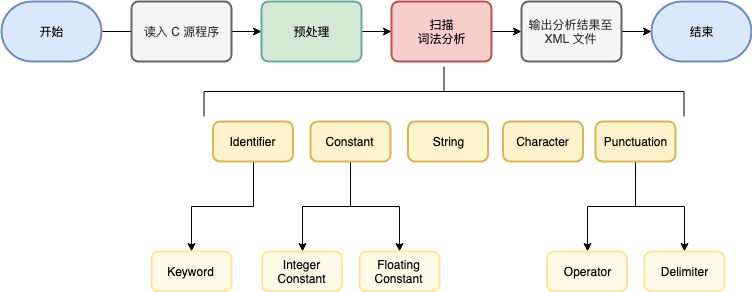
\includegraphics[width=\linewidth]{images/lexical.png}
  \caption{词法分析器的大致流程}
  \label{fig:figure1}
\end{figure}

也就是说,我们本次需要实现的模块有:

\begin{enumerate}
  \item 文件读入
  \item 程序预处理模块(去除每行前部分空格、注释等)
  \item 进行词法分析,依次识别:
  \begin{itemize}
    \item 标识符 Identifier
    \item 常量 Constant
    \begin{itemize}
        \item 整数型常量 Integer Constant
        \item 点型常量 Floating Constant
    \end{itemize}
    \item 字符 Char
    \item 字符串 String
    \item 算符 Punctuation
      \begin{itemize}
        \item 运算符 Operator
        \item 界限符 Delimiter
      \end{itemize}
  \end{itemize}
  \item 输出 XML 文件
\end{enumerate}

\subsection{具体模块的实现}

接下来,我们分别对各个模块相应的具体实现方法进行介绍。

\subsubsection{程序输入和预处理}

本次实验中的输入是一个 C 语言程序的源文件。我们从命令行读入需要处理的文件路径,处理文件内容。

\begin{minted}[linenos,frame=lines,framesep=2mm]{python}
def main():
  # Print usage if arguments are not legal
  if len(sys.argv) < 2:
    print('[Usage] ./scan.py <C source file path>')
    sys.exit(0)

  # Read file from file path taken from command line arguments
  filePath = sys.argv[1]
  with open(filePath, 'r', encoding='utf-8') as f:
    content = f.readlines()
\end{minted}

在读文件时,我使用了 \texttt{readlines()} 函数为了逐行读入文件。我们得到 \texttt{content},也就是代码的基本内容。之后,我们对读入的内容进行预处理。

\begin{minted}[linenos,frame=lines,framesep=2mm]{python}
# 主函数内的内容,预处理代码内容
code = preProcess(content)
# 预处理函数
def preProcess(content):
  code = ''
  # Trim leading white space 去掉每行最前面的空白
  for line in content:
    if line != '\n':
      code = code + line.lstrip()
    else:
      code = code + line
  return code
\end{minted}

我首先定义代码变量 \texttt{code},之后按行处理代码内容,对于每一行代码,如果代码不是空行,那么我就将这一行的代码和前面定义的 \texttt{code} 相连接,之后我们只需要处理 \texttt{code} 缓冲区内的代码内容即可。

接下来,我们利用自动机对输入字符串进行匹配来判断其输入类型。首先,我定义了下面一个指针(即当前读入字符位置)和五个识别类型:

\begin{minted}[linenos,frame=lines,framesep=2mm]{python}
# 指针查找位置
index = 0

# Token 属性
codeNum = 1
codeType = ''
codeLine = 1
codeValue = ''
codeValid = 0
\end{minted}

我维护指针 \texttt{index} 用来遍历输入代码串,利用 \texttt{codeNum}、\texttt{codeType}、\texttt{codeLine}、\\\texttt{codeValue}、\texttt{codeValid} 来分别标识:当前识别的 Token 数量、当前识别 Token 的种类、当前读到代码行数、当前识别 Token 的内容以及当前识别 Token 是否合法。

之后,我构造 \texttt{scanner()} 来对输入串进行扫描识别处理:

\begin{minted}[linenos,frame=lines,framesep=2mm]{python}
def scanner(code):
  # 当前扫描代码位置
  global index
  # 当前识别符数
  global codeNum
  # 当前代码行
  global codeLine

  # 识别到词语的类别
  global codeType
  codeType = ''
  # 识别到的词语
  global codeValue
  codeValue = ''
  # 当前识别字符
  character = code[index]
  index = index + 1

  # Ignore white space
  while character == ' ':
    character = code[index]
    index = index + 1
  ...
\end{minted}

在主函数 \texttt{main()} 中,我通过这样的方式调用扫描器:

\begin{minted}[linenos,frame=lines,framesep=2mm]{python}
# Start scanning!
global codeNum
while index <= len(code) - 1:
  scanner(code)
\end{minted}

接下来,我构建了五个自动机,分别对标识符、常量、字符、字符串和算符进行了识别。

\subsubsection{标识符 Identifier 的判断}
标识符 Identifier 是由字母、数字或下划线“\_”组成的,具体的定义大致是这样的:

\begin{equation}
\begin{split}
  identifier \rightarrow &\ identifier-nondigit \ \\ |\ & identifier\ identifier-nondigit \ \\ |\ & identifier\ digit
\end{split}
\end{equation}
\begin{equation}
  identifier-nondigit \rightarrow \ nondigit \ |\ universal-character
\end{equation}
\begin{equation}
  nondigit \rightarrow \_ \ |\ a ... z\ |\ A ... Z
\end{equation}
\begin{equation}
  digit \rightarrow 0 ... 9
\end{equation}

为了识别标识符,我确定如图 2 的状态机。

\begin{figure}[h]
  \centering
  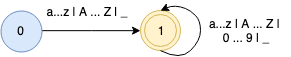
\includegraphics[width=0.45\textwidth]{images/identifier.png}
  \caption{识别标识符的状态机}
  \label{fig:2}
\end{figure}

之后,我们就可以实现对标识符的识别:

\begin{minted}[linenos,frame=lines,framesep=2mm]{python}
# Identifier!
if character.isalpha() or character == '_':
  while character.isalpha() or character.isdigit() or character == '_':
    codeValue = codeValue + character
    character = code[index]
    index = index + 1
  codeType = 'identifier'
  index = index - 1
\end{minted}

在识别了标识符之后,我们可以直接继续判断这个标识符是不是 C 语言中的关键词(Keyword)之一。我们本次实验需要判断的是 C 语言的子集,需要进行识别的关键词有这些:

\begin{center}
  \captionsetup{position=above}
  \captionof{table}{C 语言关键词表}
  \begin{tabular}{c|c|c|c|c}
    \hline
    auto & break & case & char & const \\
    continue & default & do & double & else \\
    enum & extern & float & for & goto \\
    if & inline & int & long & register \\
    restrict & return & short & signed & sizeof \\
    static & struct & switch & typedef & union \\
    unsigned & void & volatile & while \\
    \hline
  \end{tabular}
\end{center}

于是,我们维护一个关键词列表 \texttt{cKeywords},之后通过字符串匹配的方式识别标识符是否为关键词:

\begin{minted}[linenos,frame=lines,framesep=2mm]{python}
# Keyword!
for keyword in cKeywords:
  if codeValue == keyword:
    codeType = 'keyword'
    break
\end{minted}

这样我们就可以成功的识别 Token 中的标识符和关键词。

\subsubsection{常量(整形常量 Integer Constant 和浮点型常量 Floating Constant)的判断}
在 C 语言的语法中,常量 Constant 有整形和浮点型两种需要进行识别。整形常量 Integer Constant 的文法可以这样描述:

\begin{equation}
  \begin{split}
    integer-constant \rightarrow \ decimal-constant \ integer-suffix\\|\ octal-constant \ integer-suffix\\|\ hexadecimal-constant \ integer-suffix
  \end{split}
\end{equation}
\begin{equation}
  decimal-constant \rightarrow 1...9\ |\ decimal-constant\ digit
\end{equation}
\begin{equation}
  octal-constant \rightarrow 0\ |\ octal-constant\ octal-digit
\end{equation}
\begin{equation}
  \begin{split}
    hexadecimal-constant \rightarrow hexadecimal-prefix\ hexadecimal-digit\\|\ hexadecimal-constant\ hexadecimal-digit
  \end{split}
\end{equation}
\begin{equation}
  hexadecimal-prefix \rightarrow 0x\ |\ 0X
\end{equation}
\begin{equation}
  \begin{split}
    integer-suffix \rightarrow\ unsigned\ long\ |\ unsigned\ long-long\\|\ long\ unsigned\ |\ long-long\ unsigned
  \end{split}
\end{equation}

浮点型常量 Floating Constant 的文法可以这样描述:

\begin{equation}
  floating-constant \rightarrow\ decimal-floating-constant\ |\ hexadecimal-floating-constant
\end{equation}
\begin{equation}
\begin{split}
    decimal-floating-constant \rightarrow\ fractional-constant\ exp\ floating-suffix\ \\ |\ digital-seq\ exp\ floating-suffix
\end{split}
\end{equation}
\begin{equation}
\begin{split}
    hexadecimal-floating-constant \rightarrow\ hexadecimal-prefix\ \\hexadecimal-frac-constant\ binary-exp\ floating-suffix\ \\|\ hexadecimal-prefix\ hexadecimal-digit-seq\\\ binary-exp\ floating-suffix
\end{split}
\end{equation}
\begin{equation}
  exp \rightarrow\ e\ digit-seq\ |\ E\ digit-seq
\end{equation}
\begin{equation}
  sign \rightarrow\ +\ |\ -
\end{equation}
\begin{equation}
  digit-seq \rightarrow\ digit\ |\ digit-seq\ digit
\end{equation}
\begin{equation}
\begin{split}
  hexadecimal-frac-constant \rightarrow\ hexadecimal-digit-seq\ .\ \\hexadecimal-digit-seq\ |\ hexadecimal-digit-seq\ .
\end{split}
\end{equation}
\begin{equation}
  binary-exp \rightarrow\ p\ digit-seq\ |\ P\ digit-seq
\end{equation}
\begin{equation}
\begin{split}
    hexadecimal-digit-seq \rightarrow\ hexadecimal-digit-seq\ |\\\ hexadecimal-digit-seq\ hexadecimal-digit
\end{split}
\end{equation}
\begin{equation}
  floating-suffix \rightarrow\ f\ |\ F\ |\ l\ |\ L
\end{equation}

其中我们需要特别注意的是:
\begin{itemize}
  \item 整数常量中有十进制 Decimal、八进制 Octal 和十六进制 Hexadecimal 三种常量需要考虑,其中以 0 开头的是八进制数字,以 0x 或 0X 开头的是十六进制数字,其他我们都直接认为是十进制数字
  \item 浮点型常量中需要考虑科学计数法,比如 1.5e-4 就是一个合法的浮点型常量
  \item 整数常量中的后缀字符有 u、U 表示无符号整形 unsigned 和 l、L 表示长整型 long 或 long long,也就是说比如 512ull 这样的无符号长整型就是合法的十进制整型常量
  \item 浮点型常量中后缀字符有 f、F、l、L,其中 f、F 表示 float 类型的浮点型常量,没有 f、F 后缀的浮点型常量我们认为是 double 类型的;l、L 表示长浮点型常量,即比如 1.5F、4.9L 这样的浮点数是合法的
\end{itemize}

综合整形常量和浮点型常量的文法表示和注意,我们可以构造如下的自动机来识别整形和浮点型常量。

\subsubsection{字符 Character、字符串 String 的判断}
字符和字符串我们需要分别进行判断。我在这一步骤的判断是基于界限符单引号\ ' 和双引号\ " 来判断 Token 属于字符还是字符串。

我们首先利用文法描述字符常量:
\begin{equation}
  char-constant \rightarrow\ 'c-char-seq'
\end{equation}
\begin{equation}
  c-char-seq \rightarrow\ c-char\ |\ c-char-seq\ c-char
\end{equation}
\begin{equation}
  c-char \rightarrow\ all\ symbols\ other\ than\ ', \ \setminus\ and\ \setminus n\ |\ esc-seq
\end{equation}
\begin{equation}
  esc-seq \rightarrow\ \setminus'\ |\ \setminus"\ |\ \setminus?\ |\ \setminus\setminus\ |\ \setminus a\ |\ \setminus b\ |\ \setminus f\ |\ \setminus n\ |\ \setminus r\ |\ \setminus t\ |\ \setminus v
\end{equation}

字符串常量同样可以用文法表示如下:
\begin{equation}
  string-literal \rightarrow\ "s-char-seq"
\end{equation}
\begin{equation}
  s-char-seq \rightarrow\ s-char\ |\ s-char-seq\ s-char
\end{equation}
\begin{equation}
  s-char \rightarrow\ all\ symbols\ other\ than\ ', \ \setminus\ and\ \setminus n\ |\ esc-seq
\end{equation}
\begin{equation}
  esc-seq \rightarrow\ \setminus'\ |\ \setminus"\ |\ \setminus?\ |\ \setminus\setminus\ |\ \setminus a\ |\ \setminus b\ |\ \setminus f\ |\ \setminus n\ |\ \setminus r\ |\ \setminus t\ |\ \setminus v
\end{equation}

\subsubsection{算符(包括运算符 Operator 和界限符 Delimiter)的判断}
在 C 语言中,能够被识别的算符有:

\section{实验结果}

\section{实验心得体会}
通过本次实验,我重新认识了 C 语言编写的程序在编译过程中词法分析的具体方法。我不仅更加了解了标识符、常量、字符和算符的具体文法描述,还实际的利用了自动机对这些 Token 进行匹配,大致实现了一个简单的词法识别器,能够对一段 C 语言代码进行分析,得到每个识别 Token 的位置、属性和是否合法等性质。

在本次实验的词法分析中,虽然每种 Token 的文法描述都非常复杂,但是我发现,只要认真仔细的写好自动机的具体识别过程,利用 Python 来实现这个自动机还是相对简单。

同时,我也在本次实验中领略到各种不常用的 C 语言合法的语法,比如 \texttt{0777}、\texttt{0xAFull} 等八进制、十六进制整数,比如 \texttt{1.5e-4}、\texttt{0.5F} 等各种形式的浮点数,比如 \texttt{<\%}、\texttt{|=}、\texttt{...} 等不常见的算符。这让我重新了解了 C 语言的语法表示,也让我对自动机理论有了新的认识。
\end{document}